\documentclass[12pt,a4paper]{article}
%
\usepackage{graphicx}
\usepackage{helvet}

\usepackage{parskip}% http://ctan.org/pkg/parskip
\usepackage{fancyhdr}
\usepackage{titlesec}
\PassOptionsToPackage{hyphens}{url}\usepackage{hyperref}
\usepackage{apacite}

\pagestyle{fancyplain}
\fancyhf{}
\renewcommand{\headrulewidth}{0.5pt}
\renewcommand{\footrulewidth}{0.5pt}
\setlength{\headheight}{15pt}
\fancyhead[L]{}
\fancyhead[R]{}
\fancyfoot[R]{INF10101}
\fancyfoot[L]{40200819}
\fancyfoot[C]{\thepage}
\usepackage{longtable}

\renewcommand{\familydefault}{\sfdefault}
\linespread{1.5}
% Used for displaying a sample figure. If possible, figure files should
% be included in EPS format.
%
% If you use the hyperref package, please uncomment the following line
% to display URLs in blue roman font according to Springer's eBook style:
% \renewcommand\UrlFont{\color{blue}\rmfamily}

%\makeatletter
%\renewcommand\subsection{\@startsection {subsection}{1}{2mm} % name, level, indent
%                               {3pt plus 2pt minus 1pt} % before skip
%                               {3pt plus 0pt} % after skip
%                               {\normalfont\bfseries}}
%\makeatother
%\makeatletter
%\renewcommand\section{\@startsection {section}{1}{0mm} % name, level, indent
%                               {4pt plus 2pt minus 1pt} % before skip
%                               {4pt plus 0pt} % after skip
%                               {\bfseries}}
%\makeatother



\begin{document}
%

\newcommand{\HRule}{\rule{\linewidth}{0.5mm}}

\begin{titlepage}
	\begin{center}

	\HRule \\[0.4cm]
    	{\Large \bfseries INF10101 - Security Coursework\par}
	\vspace{0.2cm}
	\HRule \\[1.5cm]

	
    	\vspace{1cm}
	\begin{minipage}{0.8\textwidth}
	\begin{center} \large
        David Frame - 40200819
        	
				
   	 \end{center}
    	\end{minipage}
	
    	\begin{minipage}{1\textwidth}
    	\begin{center} \large
        
		Computing Science
    	\end{center}
    	\end{minipage}
    	
    \vspace{2cm}
    \begin{minipage}{0.8\textwidth}
	\begin{center} \large
        \emph{Word Count: 2021 words}
        	
				
   	 \end{center}
    	\end{minipage}
	
	

    	\vfill

    	% Bottom of the page
	\begin{minipage}{1\textwidth}
    	\begin{center} \large
		School of Computing
    	\end{center}
    	\end{minipage}
	
	\vspace{1cm}
    	{\large \today}


	\end{center}
\end{titlepage}

\section{Threat Context}
\subsection{The organisation, it's information assets and it's vulnerabilities}
Forthview Surgery is a large, busy medical practice situated in the ground floor of Tummel House (scenario, para 13). The GPs at the surgery are effectively partners rather than employees as they are self employed under contract to the NHS; they receive a share of the practice's profits and organise their own holidays (scenario, para 15). 

The surgery has access to a lot of information assets that could be valuable to malicious people. These information assets may include personal information about patients and staff that could be sold illegally to advertisers or used to blackmail patients with sensitive information such as their sexual health. If an attacker wanted to harm an important individual (for example a politician), their health details, such as substances that they are allergic to (scenario, para 19), could be a valuable data asset \cite{politician}. 

If money was an objective, attackers may want to sell prescription drugs on the black market. Therefore, systems dealing with prescriptions could also be information assets (scenario, para 17). Also for monetary purposes, the surgery's computing power could be an exploitable asset for cryptocurrency miners, also known as cryptojacking. A similar issue happened recently when a browser plugin named "browsealoud" was breached to allow the injection of cryptojacking scripts on NHS websites, stealing computing power from the websites' visitors \cite{cryptojacking}.

Social engineering could make these information assets vulnerable by, for example, manipulating staff into giving away patient information or prescriptions. The GPs could be sent a deceptive letter requesting a prescription, which would be a spear phishing attack (scenario, para 15). The GPs may also pose a risk if they use the Vision system (scenario, para 23) in public, as they could accidentally expose passwords and other information to onlookers.

Public access to the building could be a vulnerability, especially if a perpetrator was willing to pose as a patient to steal their personal information. In addition, the GP2GP service could be intercepted to steal information by posing as a GP who needs the patient's data (scenario, para 17). These threats could be disastrous if the perpetrator were to steal patient or staff information and sell it, or use it for other malicious purposes. It may even result in the need for thorough security and identity checks when patients enter the surgery.

The emergency care system is accessible by various parties, making the data vulnerable to many potentially manipulable people, or disgruntled employees (scenario, para 17) \cite{patientConfidentiality}. Also, overworked staff such as Dr Holloway and Dr Wells struggle to keep their administration up to date (scenario, para 14), which may cause a vulnerability if they don't update their passwords regularly. 

As the surgery is a joint data controller with the Lennox and Gilchrist pharmacy (scenario, para 19), one could make the other vulnerable in the case of a breach.

The following table lists the information assets mentioned earlier, vulnerabilities that may be exploited to access them and the consequences if they get into the wrong hands. Each consequence is labelled as a confidentiality, integrity or availability issue, following the CIA principle of information security \cite{CIA}.

\begin{center}
\begin{longtable}{ |p{0.3\textwidth}|p{0.3\textwidth}|p{0.3\textwidth}| } 
 \hline
 \textbf{Information Asset} & \textbf{Vulnerability} & \textbf{Consequences} \\ 
  \hline
 Patient and staff details & Social engineering and/or carelessness of staff & Identity theft, blackmail, GDPR breach. (Confidentiality)\\ 
  \hline
 Computing Power & Ageing Windows 2003 server (could be easy to hack into, giving access to the surgery's PCs) & Slower or unusable computers, failure of surgery equipment, compromised security which could lead to further consequences. (Availability and integrity) \\ 
 \hline
 Information about important individuals & GP2GP Interception and/or Social Engineering & Blackmail, Stalking, Violence, GDPR breach. (Confidentiality) \\ 
 \hline
 Prescription systems & Spear Phishing & Selling drugs to the black market, deaths due to altered dosages, inability to prescribe drugs when needed. (Availability and integrity) \\ 
 \hline
 Emergency care system & Social engineering and/or disgruntled employees & Inability to respond quickly to incidents, stealing of personal data. (Accessibility and confidentiality) \\
 \hline
 GP Login & Infrequent updating of passwords or carelessness in public & Criminals accessing medical records and prescription systems. (Confidentiality and integrity) \\ 
 \hline
\end{longtable}
\caption{\textit{Table 1: Information assets, vulnerabilities and consequences}}
\end{center}

\subsection{Identifying threat actors}
Due to the highly sensitive data being processed by the surgery, there could be many potential threat actors with various motivations. This section discusses three of them.

Disgruntled ex-employees can be a problem for some companies, though in this case they would be the lowest threat of the three actors. They would be unlikely to take down vital systems due to the potential harm it could inflict on innocent patients. Instead, they may steal IP or staff information as retaliation for poor treatment while they worked there. This threat may be higher than normal as the staff are contractors, so they may have less of a relationship to the other staff members - The well known 'Maroochy' case mirrors this, where a former contractor hacked into a sewage system \cite{exemployee}.

Script Kiddies are another cause for concern. Motivations vary on a person to person basis and their targets can be random \cite{scriptKiddies}, so their threat level is in the middle - they may just want to cause a bit of trouble for their own entertainment, or they might try to take data for ransom. However, even if they have sinister motivations, they would still have less resources than organised crime. 

Organised Crime is the biggest threat to most large companies, and particularly vital services such as the NHS. According to Verizon \cite{verizon}, most threats are motivated by money, which can be highly damaging by itself, but  attacks involving ransomware can have even more serious side effects. These issues vary, but in the healthcare sector they may include the loss of patient information or the inability to perform operations due to computer systems being disabled \cite{organisedCrime}.

\subsection{Goal for further analysis}
After reviewing the threat actors, it seems most appropriate to analyse organised crime as it poses the highest threat of the three. Both money and information could be goals of this threat actor, but the author ultimately chose to analyse the threat of ransomware as it recently caused a huge disaster for the NHS with WannaCry \cite{wannaCry}.

\section{Modelling the threat}

"Threat modelling can be
used as foundations for the specification of security requirements" \cite{modellingImportant}. Therefore, it is important to choose a robust and relevant model to ensure that your organisation is protected against any threats it may face.

In this case, we aim to protect against the threat of ransomware, a relatively new threat. As such, models are more important than ever to educate staff members on the dangers of this new type of virus, specifically the processes that the perpetrator will follow to infect their PCs.

The author researched various models to find one suitable for ransomware. The Cyber Kill Chain was considered, but it appears to be better suited to malware and other hidden, perimeter-based attacks \cite{AttackCKC}.

The major difference with ransomware is that it is not hidden from the victims, instead exposing itself and asking victims to pay a ransom for the decryption of their data. This unorthodox approach therefore requires a matching, unique model.

One such model is a kill chain specific to ransomware, called the Ransomware Kill Chain. It was developed by Hornet security \cite{Hornet} to help businesses plan for ransomware attacks like WannaCry, so it seems appropriate for this subject matter. See the diagram below of the Ransomware Kill Chain which shows each step of a ransomware attack.
\begin{figure}
\centering
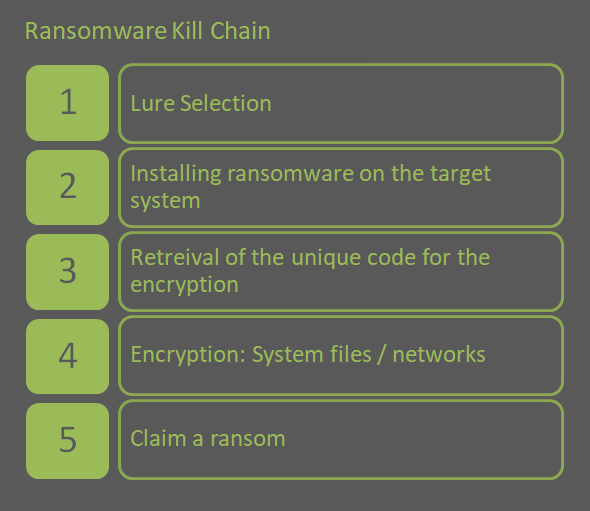
\includegraphics[width=1\textwidth]{RKCCustom.PNG}
\caption{\textit{The Ransomware Kill Chain}}
\end{figure}

\newpage
Below is a table listing the advantages and disadvantages of this approach, with points next to their counterpoints where possible.

\begin{center}
\begin{longtable}{ |p{0.45\textwidth}|p{0.45\textwidth}| } 
 \hline
 \textbf{Advantages} & \textbf{Disadvantages} \\ 
  \hline
 It allows the surgery to anticipate the stages of attack that the criminals may follow. & Attack strategies change constantly, so the model would need to keep up (this is the case with any security model). \\ 
  \hline
 Designed specifically for ransomware, making it easier to plan for this type of attack. & The specificity to ransomware means that other models would be required for comprehensive security. \\ 
 \hline
 Raises awareness, especially good for non technical staff's understanding. & The requirement for multiple models could impact understanding. \\ 
 \hline
 Based on the Cyber Kill Chain, which is a common and therefore easily implementable for those familiar with the concept. & It is not an industry standard or published model that has been 'battle tested' like the standard Cyber kill chain. \\ 
 \hline
\end{longtable}
\caption{\textit{Table 2: Advantages and disadvantages of the Ransomware Kill Chain}}
\end{center}

\section{Analysing the threat}
Attacks like WannaCry, Petya and Jaff are all examples of ransomware. Ransomware makes systems unusable until the user pays the ransom, which has the side effect of putting lives at risk in the case of computers in the health sector.

WannaCry was based on a vulnerability in older versions of Windows called 'External Blue SMB'. The vulnerability has since been patched, but as the surgery uses an 'ageing windows 2003' server (scenario, para 20), it may still be vulnerable if they haven't updated it \cite{wannaUpdate}.

Patching this issue also wouldn't protect the surgery against other ransomware, which is becoming more common in part thanks to open source encryption code that is easily accessible \cite{openRansom}.

Due to the complete data lock-down initiated by these viruses, they can be difficult to come back from without pre-emptive preparation and quick action after detection, which can be more easily done with an effective model. The table below details the stages of a ransomware attack according to the Ransomware Kill Chain.

\begin{center}
\begin{longtable}{ |p{0.3\textwidth}|p{0.6\textwidth}| } 
 \hline
 \textbf{Stage} & \textbf{Description} \\ 
  \hline
 Lure Selection & The way that the attacker will bait the victims. Often via social engineering methods such as email phishing, though fake web pages and/or advertising. These methods would download an infected file such as a PDF to the victim's machine.\\ 
  \hline
 Installing ransomware on the target system & The ransomware is installed on the victim's machine \\ 
 \hline
 Retrieval of encryption code & A unique key is fetched from a remote server that will act as the pass code to decrypt the victim's data, though this is not guaranteed. \\ 
 \hline
 Encryption: System files / Networks & The victims files are encrypted by the ransomware using the key fetched in the previous step. In some cases it will encrypt other machines on the network, which could be catastrophic for the surgery and other medical centres that it networks with - especially if it disables any medical equipment. \\ 
 \hline
 Claim a ransom & The victim is presented with a notification explaining what has happened, how much they need to pay and the method for doing so. Often a deadline is supplied to threaten victims with file deletion or price increases. The payment is usually with bitcoins as they are difficult to trace. \\ 
 \hline
\end{longtable}
\caption{\textit{Table 3: The Ransomware Kill Chain}}
\end{center}

Models are not a perfect solution. The first few stages of a model are often external and therefore not always visible to the organisation \cite{AttackCKC}. In this case, the surgery has no control over the lure selection process, the criminals will choose a method to lure staff and the surgery wouldn't know about it until they notice a phishing attempt or when their system is infected.

Therefore it is vital to train staff to understand what a phishing email/fake website/malicious advertisement may look like, and encourage them to report anything suspicious to an authoritative figure, in this case their IT manager Ben Sutherland (scenario, para 16).

Below is a table indicating the prevention and detection of ransomware at each phase of the Ransomware kill chain.

\begin{center}
\begin{longtable}{ |p{0.3\textwidth}|p{0.3\textwidth}|p{0.3\textwidth}| } 
 \hline
 \textbf{Stage} & \textbf{Prevent} & \textbf{Detect} \\ 
  \hline
 Lure Selection & Train staff to recognise various forms of phishing attempts, such as email phishing, fake websites and malicious advertisements. & Use a spam filter. Report any suspicious emails to an authority. \\ 
  \hline
 Installing ransomware on the target system & Use an antivirus program, ideally with ransomware prevention features & Report any unexpected changes to the computer, such as slowing down - this stage would be very difficult to detect \\ 
 \hline
 Retrieval of encryption code & Set up computer systems to require permission to access the internet & Keep an eye on logs for servers, flag any strange requests - especially to known ransomware sites \\ 
 \hline
 Encryption: System files / Networks & Create backups of all files and store them in another location off-network. This won't prevent files being encrypted, but can be used to bring them back. & Heavy hard drive usage as the data is encrypted, though it would be too late at this point. \\ 
 \hline
 Claim a ransom & Look for any known hacks to decrypt this variant of ransomware, which may be possible due to poor code. & Detection is easy as the ransomware exposes itself. \\ 
 \hline
\end{longtable}
\caption{\textit{Table 4: Preventing and detecting ransomware}}
\end{center}

The Ransomware Kill Chain does not cover the preparation before an attack, which is vital for the surgery to recover quickly. They would need a pre-determined plan for how to deal with attacks, including a plan for informing patients that they could have been affected, a plan to get systems back up quickly and a plan for informing the ICO within the time allowances of GDPR \cite{ICO}. They would also need to have backups that are easily accessible and off of their network.

If an attack does happen, it is important to analyse and learn from it. This would involve working out what allowed the ransomware onto the system and patching the flaw, or improving training in the case of social engineering. It would also be important to dispose of any infected and irredeemable hard drives to prevent accidental use in the future.

\section{Note for management}
Recent years have seen a huge increase in the capability and availability of technology - but also a similar increase in our reliance on it. As such, the impact of cyber crime can be catastrophic for a large company or organisation. Now consider vital services like the NHS, with a huge collection of very personal information about almost everyone in the UK. The potential for a data breach is huge and the implications are dangerous. For these reasons, cyber security is a challenging but necessary process to ensure patient safety. 

As Schneier explains, security is not a product, it is a process that is only as strong as it's weakest link \cite{processproduct}, so it is important to continually reevaluate security processes to keep up with cyber criminals.

Vulnerability assessment will allow the surgery to protect their patients proactively by anticipating threats and putting countermeasures in place. The vulnerabilities in section 1.1 should be taken into account when planning protection strategies, but they are not the only possible issues. The challenge with vulnerability assessment is that it is an ongoing process - the surgery must continually investigate and fix possible vulnerabilities to prevent breaches.

Threat modelling raises staff awareness of the various vulnerabilities highlighted by showing the attack process diagrammatically, free from jargon and other barriers of understanding.  Using a model like the Ransomware Kill Chain can also help staff decide what to do at each stage of an attack. The Ransomware Kill Chain is a good start, but again the surgery should not stop here - other models should be employed to protect against other types of attacks, such as those from insiders.

According to Guttman and Roback \cite{RiskManagement}, "Risk management is the process of assessing risk, taking steps to reduce risk to an acceptable level and maintaining that level of risk.". Risk management helps to mitigate issues by evaluating their likelihood in advance and having a reasonable risk threshold. One of the challenges of risk management is allowing staff members enough freedom, while limiting riskier activities, such as home access to patient information.

These vulnerabilities and risks can be reduced with smart staff management and use of protective technology.

Consider who has access to patient information, it should only be accessible to those that need it - the surgery has a good start with this already as the receptionist has no access to patient records (scenario, para 14).

It is vital to train staff on the dangers of social engineering. This may involve showing them examples of phishing emails and telling them how to report anything suspicious.

It is also important to handle mistakes correctly, such as staff that accidentally get viruses. Severe punishments or firing may make others more vigilant, but much less likely to come forward if they cause any issues themselves. A better approach would be to encourage employees to speak up if they see anything suspicious, with reassurance that they cannot be punished for it.

The staff must have a strategy for dealing with emergencies so that they know what to do in any situation. This could involve wiping the affected machines and using backups to restore them, using spam filters and installing antivirus programs.

\bibliographystyle{apacite}
\bibliography{Bibliography}

\end{document}
